\clearpage{\pagestyle{empty}\cleardoublepage}

\chapter{Tecnologie}
\label{chapter:second}

Nel seguente capitolo verranno presentate le tecnologie adottate per la realizzazione del progetto AirQualityInsight.
Data la natura di applicazione web del progetto, le tecnologie sono state classificate distinguendo tra quelle
utilizzate per il front-end e quelle per il back-end.

\section{Applicazioni front-end}

In questa sezione verranno presentate le principali tecnologie front-end impiegate nello sviluppo
del progetto AirQualityInsight.
L'applicazione front-end verrà sviluppata in Javascript utilizzando i seguenti framework:
\begin{itemize}
  \item Vue per lo sviluppo dell'architettura e della struttura generale dell'applicazione.
  \item Leaflet per la visualizzazione della mappa interattiva.
\end{itemize}

Di seguito, la descrizione dettagliata delle singole tecnologie.

\subsection{Vue}

Vue.js è un framework JavaScript progressivo per la costruzione di interfacce utente,
creato da Evan You nel 2014 \cite{vue2014}. Nato dall'esperienza dell'autore con AngularJS \cite{angularjs2010}
durante il suo periodo in Google, Vue è stato progettato per essere facilmente adottabile,
combinando le peculiarità di Angular e React \cite{react2013} con una curva di apprendimento più veloce
per gli sviluppatori che si interfacciano con esso.

La caratteristica distintiva di Vue risiede nella sua natura progressiva, che consente di adottarlo gradualmente in base
alle necessità del progetto. Al livello più elementare, Vue può essere utilizzato come una semplice libreria JavaScript
per arricchire pagine \acrshort{html} esistenti con funzionalità interattive. A livello intermedio invece, il framework
è in grado di gestire componenti complessi in relazione fra loro utilizzando sistemi di routing sofisticati. Infine,
al livello più avanzato, Vue permette la costruzione di \acrfull{spa} \cite{mdn2024spa} complete.

Il sistema di reattività costituisce uno dei pilastri fondamentali dell'architettura di Vue. Questo meccanismo
garantisce infatti la sincronizzazione automatica tra il modello dati e la vista, attraverso un sistema di
data binding bidirezionale, ossia un meccanismo di sincronizzazione automatica che mantiene allineati i dati tra
il modello dell'applicazione (model) e l'interfaccia utente (view) in entrambe le direzioni. Le computed properties
permettono la definizione di proprietà calcolate che si aggiornano automaticamente quando cambiano le loro dipendenze,
mentre i watchers offrono la possibilità di creare osservatori personalizzati per reagire a modifiche specifiche
dei dati.

Vue adotta un'architettura basata su componenti, in cui ciascun componente costituisce un elemento modulare e
riutilizzabile dell'interfaccia utente. I \acrfull{sfc}, caratterizzati dall'estensione \texttt{.vue},
incapsulano template \acrshort{html}, logica JavaScript e stili \acrshort{css} in un unico file,
facilitando la manutenzione e l'organizzazione del codice. La comunicazione tra componenti avviene attraverso
un sistema ben definito di props per il passaggio di dati da genitore a figlio e di eventi per la comunicazione inversa.

A livello tecnico, Vue implementa un sistema di template dichiarativo che utilizza una sintassi intuitiva. Il framework
utilizza un Virtual \acrshort{dom} per ottimizzare le prestazioni, effettuando confronti tra stati precedenti e nuovi
per minimizzare gli aggiornamenti del \acrshort{dom} reale.

L'ambiente Vue si caratterizza per la presenza di molteplici strumenti di tipologie differenti. Per la gestione e
compilazione dei progetti Vue, vengono maggiormente utilizzati Vue \acrshort{cli} \cite{vuecli2018} e
Vite \cite{vite2021}: Vue \acrshort{cli} permette la per la creazione e gestione di progetti da riga di comando,
mentre Vite rappresenta un build tool con tempi di compilazione ridotti e maggiore semplicità d'utilizzo.
Per il routing esiste Vue Router \cite{vuerouter2016}, il quale gestisce il routing nelle \acrfull{spa}.
Per la gestione centralizzata dello stato si hanno Vuex \cite{vuex2016} e Pinia \cite{pinia2021}.
Infine, per il debugging, Vue DevTools \cite{vuedevtools2016} fornisce strumenti avanzati attraverso estensioni
per browser.

L'evoluzione di Vue ha visto il passaggio da Vue 2, che ha consolidato l'adozione del framework nell'ambiente
enterprise, a Vue 3, rilasciato nel 2020. L'innovazione più significativa di questa major release è probabilmente la
Composition \acrshort{api}, che permette una migliore organizzazione della logica dei componenti e facilita la
riusabilità del codice rispetto alla Options \acrshort{api}. Inoltre, è stato migliorato il supporto nativo per il
Typescript e, con l'introduzione del supporto per il tree-shaking, sono state ridotte le dimensioni generali dei bundle.

In conclusione, Vue.js trova applicazione ideale nello sviluppo di applicazioni web moderne, dalle \acrfull{spa} alle
\acrfull{pwa}, dai dashboard amministrativi alle piattaforme e-commerce. La sua natura incrementale lo rende
particolarmente adatto per la migrazione graduale di applicazioni legacy e per la prototipazione rapida
di nuove funzionalità.

\subsection{Leaflet}

Leaflet rappresenta una delle librerie JavaScript open-source più popolari per la creazione di mappe interattive
ottimizzate per dispositivi mobili e l'integrazione di funzionalità cartografiche nelle applicazioni web.
Sviluppata inizialmente da Vladimir Agafonkin nel 2011 \cite{agafonkin2011leaflet} è stata successivamente mantenuta da
una comunità attiva di sviluppatori per la cartografia digitale.

I punti cardine di Leaflet sono la semplicità, l'efficienza e l'usabilità, qualità che lo rendono uno strumento di larga
diffusione per sviluppatori che necessitano di implementare mappe interattive senza la complessità di librerie più
pesanti, grazie anche ad un footprint di soli 39 KB di JavaScript compresso \cite{leafletnpm2024}.

L'architettura modulare di Leaflet costituisce uno dei suoi principali punti di forza. Tale libreria è stata infatti
progettata seguendo il principio della responsabilità singola (\acrshort{srp}), dove ogni componente gestisce
solo alcuni aspetti specifici della funzionalità cartografica. Questa approccio consente di scegliere di utilizzare
solo i moduli necessari per il proprio progetto, riducendo così l'impatto sulle prestazioni e
facilitando la manutenzione del codice.

Le funzionalità core di Leaflet includono la gestione di layer cartografici multipli, il supporto per vari formati di
tile server, la gestione di marker personalizzabili, popup informativi, controlli di navigazione e zoom interattivo.
La libreria supporta nativamente i più comuni sistemi di proiezione cartografica, con particolare attenzione alla
proiezione Web Mercator utilizzata dalla maggior parte dei servizi di tile moderni come \acrfull{osm} e Google Maps.

È possibile inoltre installare moduli accessori (plugin) sviluppati da terzi per integrare funzionalità aggiuntive.
Tali moduli vengono realizzati, mantenuti e resi disponibili dalla comunità open source. Questi vanno ad estendere le
funzionalità base della libreria, ad esempio, aggiungendo supporto per clustering di marker, drawing tools, integrazione
con servizi di geocoding, visualizzazione di heatmap, gestione di dati GPX e altro ancora. Questa modularità permette di
costruire applicazioni cartografiche complesse partendo da una base leggera e aggiungendo solo le funzionalità
effettivamente necessarie.

Dal punto di vista delle prestazioni, Leaflet implementa diverse ottimizzazioni per garantire un'esperienza
utente fluida. Il sistema di gestione dei tile implementa strategie di caching e lazy loading, caricando solo le
porzioni di mappa effettivamente presenti nell'area di visualizzazione. Il rendering dei marker è ottimizzato attraverso
tecniche di virtualizzazione che gestiscono efficientemente svariati punti disegnati sulla mappa senza appesantire
le prestazioni di scrolling e zoom.

L'\acrshort{api} di Leaflet offre un'interfaccia intuitiva e ben documentata che segue convenzioni JavaScript moderne.
La libreria supporta sia approcci programmatici tradizionali che pattern più moderni come la programmazione funzionale e
l'utilizzo di Promise per operazioni asincrone. L'integrazione con framework JavaScript contemporanei come Vue.js,
React e Angular è facilitata da wrapper specifici e da una architettura event-driven che si integra naturalmente con i
sistemi di reattività di questi framework.

La compatibilità cross-platform di Leaflet consente di supportare i browser moderni desktop e mobile.
La libreria gestisce automaticamente le differenze tra dispositivi touch e mouse, offrendo un'esperienza di navigazione
ottimizzata per ogni tipo di interfaccia.

Dal punto di vista della personalizzazione, Leaflet offre un controllo granulare sull'aspetto e il comportamento
delle mappe. Il sistema di styling basato su \acrshort{css} permette di personalizzare completamente l'aspetto
dei controlli, marker e popup, mentre l'\acrshort{api} JavaScript consente di definire
comportamenti  interattivi complessi.
La libreria supporta la creazione di marker personalizzati utilizzando \acrshort{html}, \acrshort{css} e \acrshort{svg},
permettendo la realizzazione di interfacce cartografiche su misura.

L'integrazione con servizi di tile esterni è una delle principali caratteristiche del framework, che consentono di
supportare nativamente servizi come OpenStreetMap, Google Maps, HERE ed altri.
Questa flessibilità permette agli sviluppatori di scegliere il provider di tile più adatto alle proprie esigenze
in termini di qualità, copertura geografica e costi, mantenendo la stessa \acrshort{api} di sviluppo.

La libreria dei dati geografici supporta il formato GeoJSON nativo, permettendo la visualizzazione di geometrie
complesse come poligoni, linee e punti direttamente da dati strutturati, come le aree comunali ed i confini
territoriali ed amministrativi di regioni, province ed altre suddivisioni geografiche.
L'integrazione con servizi \acrshort{rest} e \acrshort{api} geografiche è semplificata dalla gestione intrinseca di
richieste \acrshort{ajax} e dalla capacità di processare dati in tempo reale.

La community di Leaflet mantiene attivo il core della libreria e contribuisce con supporto tecnico, numerosi plugin,
tutorial, esempi d'utilizzo ed una documentazione ufficiale completa ed aggiornata.

In termini di performance e scalabilità, Leaflet gestisce elasticamente applicazioni di varia natura e dimensione.
Per le applicazioni più semplici, la libreria offre una soluzione plug-and-play che richiede configurazione minima
per installare le sole funzionalità necessarie, in modo da migliorare l'esperienza d'utilizzo.

Il seguente esempio \ref{lst:leaflet} mostra come sia possibile realizzare una mappa con tile \acrfull{osm}
centrata su Piazza Maggiore (Bologna), ottenendo la mappa mostrata in figura \ref{fig:leaflet}:

\begin{lstlisting}[caption={Mappa Bologna con Leaflet}, label=lst:leaflet]
  // Coordinates of Piazza Maggiore
  const lat = 44.4939;
  const lng = 11.3426;

  const map = L.map('map').setView([lat, lng], 13);

  // Tiles layer (OpenStreetMap)
  L.tileLayer('https://{s}.tile.openstreetmap.org/{z}/{x}/{y}.png', {
    maxZoom: 19,
    attribution: '<a href="http://www.openstreetmap.org/copyright">OpenStreetMap</a>'
  }).addTo(map);

  // Current position marker
  const marker = L.marker([lat, lng]).addTo(map);

  // Marker popup
  marker.bindPopup(`
    <div style="text-align: center;">
      <h4>Piazza Maggiore, Bologna</h4>
      <p>Lat: ${lat}</p>
      <p>Lng: ${lng}</p>
    </div>
  `).openPopup();

  // Circle on area
  L.circle([lat, lng], {
    color: 'red',
    fillColor: '#f03',
    fillOpacity: 0.2,
    radius: 1000 // meters
  }).addTo(map);

  // Optional controls
  L.control.scale({
    imperial: false,
    metric: true
  }).addTo(map);
\end{lstlisting}

\begin{figure}[H]
  \centering
  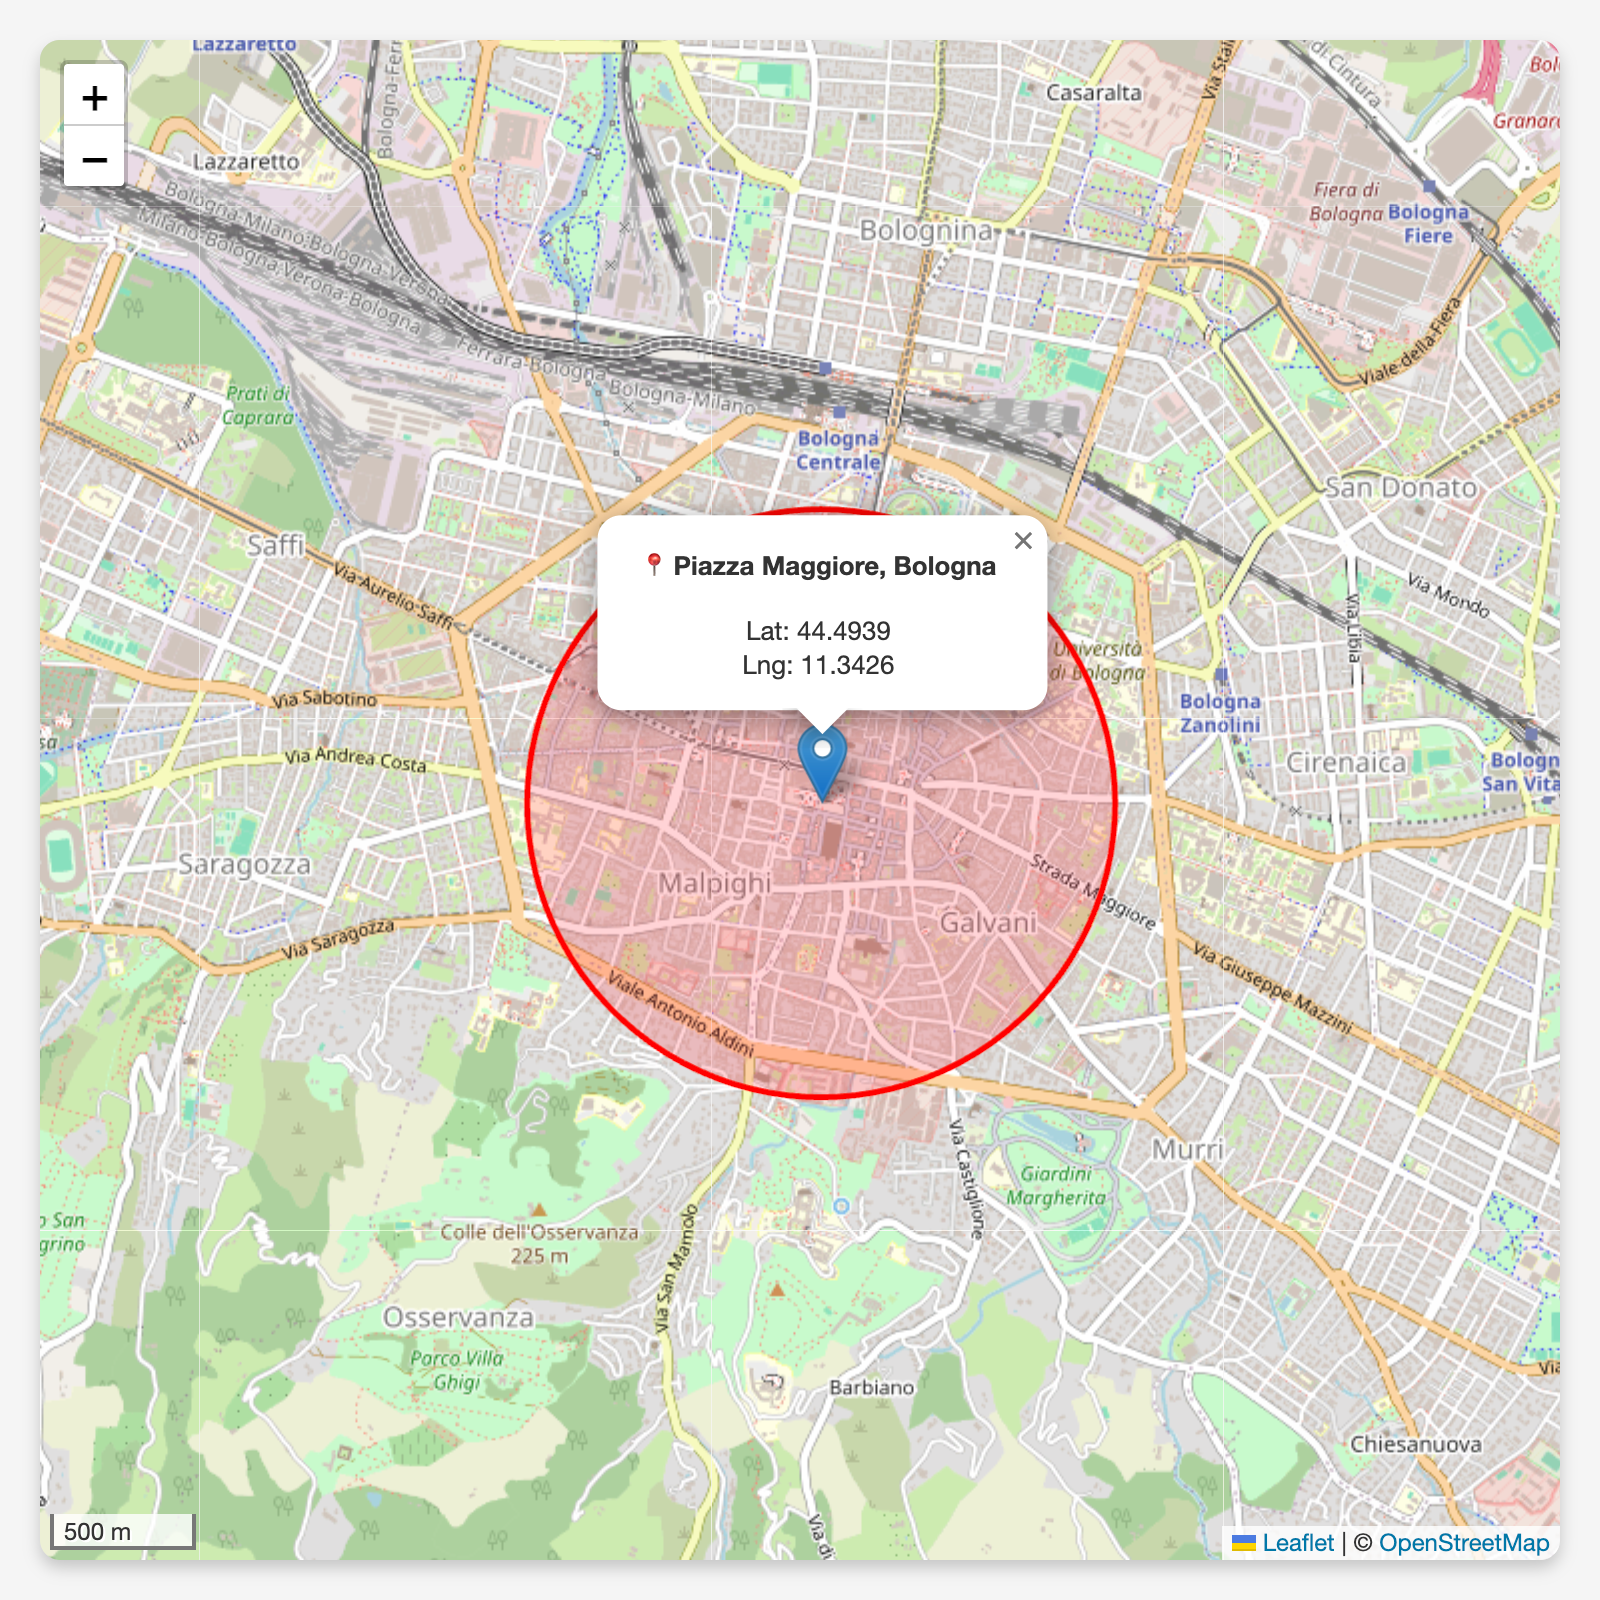
\includegraphics[width=\textwidth]{leaflet.png}
  \caption{Piazza Maggiore, Bologna}
  \label{fig:leaflet}
\end{figure}

In conclusione, Leaflet si posiziona come una soluzione affidabile per l'integrazione di funzionalità cartografiche
in applicazioni web moderne. Combinando leggerezza, potenza, estensibilità e facilità d'uso diventa una scelta indicata
per sviluppatori che necessitano di implementare mappe interattive performanti e personalizzabili, dal prototipo rapido
all'applicazione complessa.

\section{Applicazioni back-end}

In questa sezione verranno presentate le principali tecnologie back-end impiegate nello sviluppo del progetto
AirQualityInsight.

Verranno utilizzati Node.js per realizzare il server, Python per simulare i dispositivi di misurazione della
qualità dell'aria, Kafka come broker dei messaggi e MongoDB per mantenere un database documentale delle registrazioni.

\subsection{Node.js}

Node.js è un runtime system open-source multipiattaforma costruito sul motore JavaScript V8
di Google Chrome \citep{capan_2013_nodejs}. A differenza dei tradizionali ambienti JavaScript che operano esclusivamente
nel browser, Node.js permette l'esecuzione di codice JavaScript lato server, abilitando lo sviluppo di applicazioni web
complete utilizzando un unico linguaggio di programmazione.

Le principali caratteristiche di Node.js sono l'adozione di un paradigma event-driven,
un approccio non-blocking I/O ed un processo single-threaded. Il modello di programmazione orientato agli eventi
consente di gestire efficientemente operazioni asincrone basate sulla manifestazione di determinati eventi.
Le operazioni di input e di output non bloccanti migliorano le performance dell'applicativo.
L'uso di un singolo thread principale con un event loop riduce la complessità della gestione della concorrenza.

Il seguente esempio \ref{lst:node-server} mostra come creare un server \acrshort{http} minimale utilizzando Node.js:

\begin{lstlisting}[caption={Server \acrshort{http} base in Node.js}, label=lst:node-server]
const http = require('http');

const server = http.createServer((req, res) => {
  res.writeHead(200, {'Content-Type': 'text/plain'});
  res.end('Hello world!');
});

const PORT = 3000;
server.listen(PORT, () => {
  console.log(`Server listening on port ${PORT}`);
});
\end{lstlisting}

Node.js offre ampie funzionalità per l'interazione con il file system.
L'esempio seguente \ref{lst:node-fs} dimostra la lettura asincrona di un file:

\begin{lstlisting}[caption={Lettura asincrona di file}, label=lst:node-fs]
const fs = require('fs');

// Asynchronous reading
fs.readFile('file.txt', 'utf8', (err, data) => {
  if (err) {
    console.error('Error in file reading:', err);
    return;
  }
  console.log('File content:', data);
});

// Synchronous reading (not file for large files)
try {
  const data = fs.readFileSync('example.txt', 'utf8');
  console.log('File content:', data);
} catch (err) {
  console.error('Error in file reading:', err);
}
\end{lstlisting}

L'architettura di Node.js si basa sul concetto di event loop, un meccanismo che permette di gestire multiple operazioni
I/O senza bloccare l'esecuzione del programma principale \citep{nodejs_docs_2023}. Questo approccio lo rende
particolarmente adatto per applicazioni che richiedono alta concorrenza con operazioni I/O intensive,
come \acrshort{api} \acrshort{rest}, applicazioni real-time su dispositivi distribuiti e microservizi.

Le performance di Node.js sono generalmente migliori rispetto ai server tradizionali multi-threaded per applicazioni
I/O-bound, grazie alla riduzione dell'overhead dovuto al context switching tra thread e alla gestione efficiente della
memoria. Questo poiché i sistemi tradizionali adottano tecniche di gestione delle richieste creando un nuovo thread
per ogni nuova connessione, mentre Node.js, operando su un singolo thread ed utilizzando chiamate I/O non bloccati,
riesce a supportare un maggior numero di richieste concorrenti nell'event loop.

Quello che ha reso popolare tale framework è la praticità e la versatilità che lo contraddistinguono.
Risulta infatti una buona scelta nel realizzare velocemente applicazioni web scalabili, grazie alla sua capacità
di gestire un numero elevato di connessioni simultanee.

Node.js dispone di un gestore di pacchetti chiamato ``\acrshort{npm}'' (\acrlong{npm}), il quale fornisce un insieme
di librerie e componenti riutilizzabili e disponibili al pubblico, facilmente installabili tramite un repository online,
con gestione delle versioni e delle dipendenze. Tali librerie sono accessibili attraverso uno strumento
command-line dedicato.

I moduli principali sono:
\begin{itemize}
  \item Express, un framework di sviluppo web \cite{express_js};
  \item Socket.io, un componente server-side di due WebSocket components comuni \cite{socket_io};
  \item Mongodb, che fornisce \acrshort{api} per l'omonimo database \cite{mongodb};
  \item Redis, un sistema di caching \cite{redis}.
\end{itemize}
È possibile per chiunque realizzare e pubblicare la propria libreria su \acrfull{npm}.

In conclusione, Node.js rappresenta una soluzione moderna e efficace per lo sviluppo di applicazioni server-side,
disponendo di una vasta scelta di librerie disponibili attraverso \acrfull{npm} ed una community attiva.
La sua architettura event-driven e le performance elevate lo rendono una scelta ideale per molte tipologie
di applicazioni web moderne.

\subsubsection{\acrshort{wot}}

Il Web of Things (\acrshort{wot}) rappresenta un paradigma architetturale che estende i principi del \acrshort{www}
all'\acrshort{iot}, permettendo l'interoperabilità tra dispositivi eterogenei attraverso standard
web consolidati~\cite{w3c-wot-td}. L'implementazione analizzata trasforma sensori di qualità dell'aria in
\textit{Things} web-accessibili, seguendo le specifiche \acrshort{w3c} e utilizzando l'ontologia
\acrfull{saref}~\cite{saref-ontology}. Ogni sensore fisico viene quindi trasformato in una risorsa web
identificabile univocamente, accessibile attraverso protocolli \acrshort{http} standard e descritta mediante metadati
strutturati secondo il vocabolario \acrshort{wot}. Questa approccio garantisce l'interoperabilità semantica e
l'integrazione seamless con applicazioni web esistenti.

L'architettura utilizza le \acrfull{td} come elemento centrale, conformi alla specifica \acrshort{w3c} \acrshort{wot}
\acrlong{td} v1.1~\cite{w3c-wot-td}. La struttura della \acrshort{td} include diversi componenti fondamentali
che definiscono l'identità, le capacità e le modalità di interazione del dispositivo. Ogni sensore viene identificato
univocamente attraverso \acrshort{uri} strutturati (urn:sensor:air-quality:\$\{sensor\_id\}) e classificato
semanticamente usando il tipo saref:Sensor.

Il contesto semantico integra il vocabolario \acrshort{wot} standard con l'ontologia \acrshort{saref},
facilitando l'interpretazione automatica delle funzionalità del dispositivo. Le proprietà modellano
parametri ambientali con schemi di dati precisi che includono tipo, unità di misura e range di validità.

La directory \acrshort{wot} (\texttt{/wot/things}) supporta il discovery automatico dei dispositivi,
fornendo informazioni sommarie su identità, stato operativo e ultimo contatto.
Le notifiche proattive via WebSocket mantengono sincronizzate le applicazioni client senza polling periodico.

L'implementazione rispetta le specifiche \acrshort{w3c} \acrshort{wot}~\cite{w3c-wot-architecture}, utilizzando
vocabolari semantici standard e implementando gli elementi necessari.
L'uso dell'ontologia \acrshort{saref}~\cite{saref-ontology} aggiunge un layer semantico che facilita
l'interoperabilità con sistemi di building automation e smart city.

La separazione tra modello logico (\acrlong{td}) e implementazione fisica (sensori hardware) facilita l'evoluzione
dell'architettura e l'integrazione di nuove tipologie di dispositivi, confermando la validità del paradigma
\acrshort{wot} per applicazioni \acrshort{iot} di larga scala e garantiscono compatibilità
con toolchain \acrshort{wot} esistenti e scalabilità orizzontale~\cite{guinard-wot}.

\subsection{Python}

Python è un linguaggio di programmazione di alto livello, interpretato e multi-paradigma.
È stato creato da Guido Van Rossum e rilasciato per la prima volta nel 1991 \citep{van_rossum_1995}.
Il nome deriva dalla serie televisiva britannica "Monty Python's Flying Circus", riflettendo l'approccio creativo
che caratterizza l'intera filosofia del linguaggio.

La filosofia di Python è codificata nel famoso "Zen of Python" di Tim Peters, un insieme di principi guida
che enfatizzano la leggibilità, la semplicità e la qualità del codice. Tra questi principi spicca il motto
\textit{"Beautiful is better than ugly"} e \textit{"Simple is better than complex"}, che hanno influenzato profondamente
la progettazione del linguaggio e la sua evoluzione nel corso degli anni \citep{peters_2004}.

Uno degli elementi che contraddistinguono Python rispetto ad altri linguaggi di programmazione è l'assenza di parentesi
graffe per delimitare i blocchi di codice, ma bensì l'utilizzo dell'indentazione stessa. Tale caratteristica ha promosso
l'apprendimento del linguaggio a programmatori alle prime armi, che hanno potuto così concentrarsi maggiormente sul
contenuto del codice grazie alla sua forma più pulita e leggibile.

Il supporto di diversi modelli di programmazione da parte di Python lo ha reso un linguaggio versatile e popolare.
Si possono infatti scegliere approcci procedurali per script semplici, orientati agli oggetti per applicazioni più
complesse o funzionali per elaborazioni matematiche più avanzate. Questa flessibilità permette di scegliere il paradigma
migliore per il problema specifico da risolvere.

Una peculiarità del linguaggio Python è il concetto dove tutto è un oggetto, inclusi numeri, stringhe,
funzioni e persino le classi stesse. Tale uniformità concettuale semplifica notevolmente il modello mentale necessario
per comprendere il linguaggio, facilitando quindi l'apprendimento di concetti avanzati.

Il sistema di tipizzazione è forte (strong typing) ed eseguito a run-time (dynamic typing), evitando così errori comuni
dipesi dalle operazioni implicite tra tipi incompatibili. È stato introdotto il supporto per type hints, permettendo
di annotare esplicitamente i tipi delle variabili e dei parametri delle funzioni. Queste annotazioni, pur non
influenzando l'esecuzione del programma, migliorano significativamente la leggibilità del codice e abilitano strumenti
di analisi statica per la rilevazione precoce di errori di tipo.

Python gestisce in autonomia la memoria allocata grazie ad un sistema garbage collector.
Questo solleva il programmatore dalla necessità di gestire manualmente l'allocazione e la deallocazione della memoria,
riducendo drasticamente i bug legati alla gestione delle risorse. Il garbage collector rappresenta un utile strumento
che, sfruttando il reference counting ed integrato con un rilevatore di cicli, permette di individuare e segnalare
riferimenti circolari.

Anche se spesso viene inteso come linguaggio interpretato, Python in realtà non converte direttamente
il codice sorgente in linguaggio macchina, ma passa prima una fase di pre-compilazione bytecode, evitando di
reinterpretare integralmente il codice e migliorando le prestazioni.

L'ecosistema di Python è arricchito dal \acrfull{pypi}, un repository centrale che ospita centinaia di migliaia di
pacchetti di terze parti \citep{pypi_2023}. Viene così  praticamente ricoperto ogni dominio applicativo,
dalla sviluppo web all'intelligenza artificiale, dall'analisi dei dati alla computer vision.

Il sistema di gestione dei pacchetti, principalmente attraverso pip, rende estremamente semplice l'installazione e la
gestione delle dipendenze. L'introduzione di strumenti come virtualenv e, più recentemente, pipenv e poetry,
ha ulteriormente migliorato la gestione degli ambienti di sviluppo isolati, permettendo di evitare conflitti
tra diverse versioni delle librerie. Questo risulta molto comodo qualora si lavori a progetti che utilizzando versioni
differenti delle dipendenze.

La libreria standard provvede un ricco numero di moduli base, come quelli per le operazioni su file system, networking,
regex, database, threading, e molto altro. Questa completezza riduce la necessità di dipendenze esterne per molte
operazioni comuni.

Uno dei campi in cui il linguaggio è maggiormente usato è quello scientifico, dove librerie come NumPy e SciPy
hanno trasformato Python in uno strumento fondamentale per il calcolo numerico,
fornendo strutture dati efficienti e algoritmi ottimizzati per operazioni matematiche complesse.
Pandas ha rivoluzionato l'analisi dei dati, offrendo strutture dati potenti per la manipolazione e l'analisi
di dataset strutturati.

Il seguente esempio \ref{lst:measurements} mostra come sia possibile generare misurazioni aleatorie in Python:

\begin{lstlisting}[caption={Generazione di misurazioni aleatorie in Python}, label=lst:measurements]
import random
import numpy as np
from datetime import datetime, timedelta

class MeasurementGenerator:
  def __init__(self):
    self.sensors = {
      'temperature': {'min': 15, 'max': 35, 'unit': 'C'},
      'humidity': {'min': 30, 'max': 90, 'unit': '%'},
      'pressure': {'min': 990, 'max': 1030, 'unit': 'hPa'}
    }

  def generate_measurement(self, sensor_type):
      config = self.sensors[sensor_type]
      value = random.uniform(config['min'], config['max'])
      return {
        'timestamp': datetime.now().isoformat(),
        'sensor': sensor_type,
        'value': round(value, 2),
        'unit': config['unit']
      }

  def generate_time_series(self, sensor_type, hours=24, interval_minutes=60):
    measurements = []
    start_time = datetime.now() - timedelta(hours=hours)

    for i in range(0, hours * 60, interval_minutes):
      timestamp = start_time + timedelta(minutes=i)
      config = self.sensors[sensor_type]

      base_value = (config['min'] + config['max']) / 2
      daily_variation = 5 * np.sin(2 * np.pi * i / (24 * 60))
      noise = random.gauss(0, 1)
      value = base_value + daily_variation + noise

      measurements.append({
        'timestamp': timestamp.isoformat(),
        'sensor': sensor_type,
        'value': round(np.clip(value, config['min'], config['max']), 2),
        'unit': config['unit']
      })

    return measurements

if __name__ == '__main__':
  generator = MeasurementGenerator()

  single_measurement = generator.generate_measurement('temperature')
  print(f"Single: {single_measurement}")

  time_series = generator.generate_time_series('temperature', hours=12)
  print(f"Generated {len(time_series)} measurements")
  print(f"First: {time_series[0]}")
  print(f"Last: {time_series[-1]}")
\end{lstlisting}

Eseguendo il codice riportato nell'esempio \ref{lst:measurements} si può ottenere un output come riportato
in lista \ref{lst:measurements-output}:
\begin{lstlisting}[caption={Output di esempio ottenuto dalla generazione di misurazioni aleatorie in Python},
  label=lst:measurements-output]
  Single: {'timestamp': '2025-08-28T18:55:41.327822', 'sensor': 'temperature', 'value': 30.71, 'unit': 'C'}
  Generated 12 measurements
  First: {'timestamp': '2025-08-28T05:55:41.327850', 'sensor': 'temperature', 'value': 25.79, 'unit': 'C'}
  Last: {'timestamp': '2025-08-28T22:55:41.327850', 'sensor': 'temperature', 'value': 26.01, 'unit': 'C'}
\end{lstlisting}

Anche nello sviluppo web, Python rimane una delle scelte preferire dagli sviluppatori, i quali possono usare framework
come Django e Flask \citep{django_2023, flask_2023} per realizzare le proprie applicazioni web.
Fra i due, Flask risulta più minimale e flessibile per progetti che richiedono un controllo più granulare
dell'architettura, mentre Django include tutto il necessario per sviluppare sistemi complessi.

Il seguente esempio \ref{lst:flask} mostra come sia possibile realizzare un semplice server usando Flask:

\begin{lstlisting}[caption={Server Flask base in Python}, label=lst:flask]
from flask import Flask, jsonify, request

app = Flask(__name__)

users = [
  {"id": 1, "name": "John", "email": "john@example.com"},
  {"id": 2, "name": "Jane", "email": "jane@example.com"}
]

@app.route('/')
def home():
  return {"message": "Flask server running", "users_count": len(users)}

@app.route('/api/users', methods=['GET'])
def get_users():
  return jsonify(users)

@app.route('/api/users/<int:user_id>', methods=['GET'])
def get_user(user_id):
  user = next((u for u in users if u["id"] == user_id), None)
  if user:
    return jsonify(user)
  return jsonify({"error": "User not found"}), 404

@app.route('/api/users', methods=['POST'])
def create_user():
  data = request.get_json()
  if not data or 'name' not in data or 'email' not in data:
    return jsonify({"error": "Name and email required"}), 400

  new_user = {
    "id": max([u["id"] for u in users]) + 1,
    "name": data["name"],
    "email": data["email"]
  }
  users.append(new_user)
  return jsonify(new_user), 201

if __name__ == '__main__':
  app.run(debug=True, port=5000)
\end{lstlisting}

Eseguendo il codice riportato nell'esempio \ref{lst:flask} si può ottenere un output come riportato
in lista \ref{lst:flask-output}:
\begin{lstlisting}[caption={Output di esempio ottenuto dall'interazione con le rotte disposte dal server web in Flask},
  label=lst:flask-output]
  // Main url
  curl 127.0.0.1:5000
  {
    "message": "Flask server running",
    "users_count": 2
  }

  // Get all users
  curl 127.0.0.1:5000/api/users
  [
    {
      "email": "john@example.com",
      "id": 1,
      "name": "John"
    },
    {
      "email": "jane@example.com",
      "id": 2,
      "name": "Jane"
    }
  ]

  // Show informations about user #1
  curl 127.0.0.1:5000/api/users/1
  {
    "email": "john@example.com",
    "id": 1,
    "name": "John"
  }

  // Show informations about user #2
  curl 127.0.0.1:5000/api/users/2
  {
    "email": "jane@example.com",
    "id": 2,
    "name": "Jane"
  }

  // Create new user
  curl -X POST http://127.0.0.1:5000/api/users \
    -H "Content-Type: application/json" \
    -d '{"name": "Mario Rossi", "email": "mario.rossi@example.com"}'
  {
    "email": "mario.rossi@example.com",
    "id": 3,
    "name": "Mario Rossi"
  }
\end{lstlisting}


L'approccio "pythonic" enfatizza la leggibilità del codice e la rapidità di sviluppo, permettendo di creare prototipi
funzionali in tempi molto brevi e di scalare gradualmente verso applicazioni enterprise.

Sempre nel campo scientifico, Python è diventato il linguaggio de-facto per data science e machine learning,
grazie alle librerie specializzate. TensorFlow e PyTorch, ad esempio, hanno reso accessibili le tecniche di
deep learning senza il bisogno di avere nozioni approfondite di matematica avanzata.

Un altro campo in cui il linguaggio è fortemente utilizzato è quello delle DevOps e dell'amministrazione di sistemi,
grazie alla capacità di interagire facilmente con il sistema operativo, nel processare file di testo, interfacciarsi
con database e \acrshort{api} \acrshort{rest}. Viene infatti scelto per automatizzare processi ripetitivi,
creare pipeline di elaborazione dati ed integrazione di sistemi eterogenei, settori dove la rapidità di sviluppo e la
manutenibilità del codice sono cruciali.

Python rimane uno dei linguaggi più popolari e trasversali, godendo di una forte comunità che ne segue gli sviluppi e lo
aggiorna in modo continuativo, con rilasci annuali che introducono nuove funzionalità e miglioramenti delle performance.
L'adozione crescente in settori come l'intelligenza artificiale, l'\acrfull{iot} e l'edge computing suggerisce che
Python rimarrà rilevante e in continua evoluzione, adattandosi alle esigenze di un panorama tecnologico
in rapido cambiamento.

\subsection{Kafka}

Apache Kafka è una piattaforma di streaming distribuito basato su Java e Scala, progettata per gestire flussi di dati
in tempo reale su larga scala \cite{narkhede2017kafka}. Sviluppato originariamente da LinkedIn e successivamente
donato alla Apache Software Foundation nel 2011, Kafka ha acquisito presto popolarità nel panorama
della messaggistica e del processing di eventi in sistemi distribuiti \cite{garg2013apache}.

La filosofia di Kafka si basa sul concetto di event streaming, dove i dati vengono trattati come una sequenza immutabile
di eventi che possono essere pubblicati, memorizzati e processati in tempo reale \cite{stopford2018designing}.
Questo paradigma si discosta significativamente dai tradizionali message broker, offrendo persistenza duratura,
elevata throughput e capacità di replay dei messaggi, caratteristiche fondamentali per architetture moderne
basate su microservizi e event-driven architecture.

L'architettura distribuita di Kafka consente la gestione in tempo reale di grandi volumi di dati,
rendendolo una valida scelta in campi quali analytics, monitoring, fraud detection e real-time recommendation systems
\cite{kreps2014kafka}. Il sistema organizza i dati in topic, entità logiche che rappresentano categorie di messaggi
correlati \cite{narkhede2017kafka}. Ogni topic è suddiviso in partition, unità fisiche di parallelizzazione
che permettono la distribuzione del carico e la scalabilità orizzontale del sistema.

Il modello di persistenza di Kafka utilizza un commit log distribuito, dove ogni messaggio viene assegnato a un offset
sequenziale all'interno di una partizione \cite{garg2013apache}. Questa struttura garantisce l'ordinamento dei messaggi
all'interno di ciascuna partizione e permette un accesso efficiente, sia sequenziale che random, ai dati storici.
La persistenza è implementata attraverso segment files ottimizzati per operazioni append-only, minimizzando la latenza
di scrittura e massimizzando la throughput.

I broker Kafka formano un cluster distribuito che gestisce la replica dei dati attraverso il meccanismo di
leader-follower replication \cite{stopford2018designing}. Ogni partizione ha un broker leader che gestisce tutte le
operazioni di lettura e scrittura, mentre i follower mantengono copie sincronizzate dei dati. Il sistema di elezione
del leader, basato su Apache ZooKeeper (e successivamente su KRaft metadata management),
garantisce alta disponibilità e fault tolerance.

Il modello publish-subscribe di Kafka si basa sull'interazione tra produttori, che pubblicano messaggi sui
topic, e consumatori, che leggono e processano questi messaggi \cite{kreps2014kafka}.
I produttori possono configurare diverse strategie di partitioning, utilizzando chiavi di partizionamento per garantire
che messaggi correlati vengano sempre inviati alla stessa partizione, preservando l'ordinamento temporale.

Kafka supporta diverse semantiche di delivery \cite{narkhede2017kafka}: la semantica at-least-once garantisce che
ogni messaggio venga consegnato almeno una volta, ma può comportare duplicazioni; la semantica at-most-once assicura
l'assenza di duplicati ma può causare perdite di messaggi in caso di failure; la semantica exactly-once,
introdotta nelle versioni più recenti, combina transazioni e idempotenza per garantire elaborazione esatta dei messaggi.

I consumer groups rappresentano un meccanismo di parallelizzazione del consumo di messaggi \cite{garg2013apache}.
Ogni consumer all'interno di un gruppo riceve messaggi da un sottoinsieme delle partizioni del topic,
permettendo scalabilità orizzontale del processing. Il consumer group rebalancing automatico redistribuisce
le partizioni tra i consumatori attivi, favorendo load balancing dinamico e fault tolerance.

Kafka Streams costituisce una libreria client per il processing di stream di dati che elimina la necessità di framework
esterni per elaborazioni in tempo reale \cite{stopford2018designing}. Questa libreria implementa il paradigma di stream
processing attraverso topology di trasformazioni che possono includere operazioni di filtering, mapping,
aggregation e joining tra stream differenti.

La scalabilità orizzontale di Kafka è limitata principalmente dal numero di partizioni per topic, che determina il
massimo grado di parallelismo achievable \cite{narkhede2017kafka}. L'aggiunta di broker al cluster permette
di aumentare la capacità di storage e processing, ma richiede careful planning del numero di partizioni e della
strategia di replica. Il processo di partition reassignment può essere utilizzato per bilanciare il carico
tra broker esistenti e nuovi.

Kafka si rivela particolarmente efficace in architetture event-driven dove la decoupling tra componenti e la capacità
di replay degli eventi sono requisiti fondamentali \cite{stopford2018designing}.
Pattern architetturali come Event Sourcing, \acrfull{cqrs} e Saga pattern sono indicati per tale strumento.

I casi d'uso tipici di Kafka includono real-time analytics, log aggregation, metrics collection, stream processing
per machine learning e data pipeline per data lake e data warehouse \cite{kreps2014kafka}.
La capacità di Kafka di fungere sia da message broker che da storage system può essere sfruttata in architetture
dove i dati devono essere processati da multiple applicazioni con diverse temporal requirements.

\subsection{MongoDB}

MongoDB è uno dei database NoSQL orientati ai documenti più noti ed utilizzati \cite{chodorow2013mongodb}.
Sviluppato inizialmente da 10gen (ora MongoDB Inc.) nel 2009, questo database ha rivoluzionato il modo in cui
gli sviluppatori approcciano la persistenza dei dati, offrendo un'alternativa flessibile e scalabile
ai tradizionali database relazionali \cite{banker2011mongodb}.

La filosofia alla base di MongoDB si discosta significativamente dal paradigma relazionale in favore di un modello
basato su documenti \acrfull{bson} che permette una maggiore flessibilità nella strutturazione
dei dati \cite{plugge2010mongodb}. Questa caratteristica consente agli sviluppatori di memorizzare
oggetti complessi e annidati senza la necessità di normalizzazione, tipica dei database SQL tradizionali.

L'architettura di MongoDB si avvale di un approccio document-oriented, dove ogni record è rappresentato come
un documento flessibile che può contenere campi di diversi tipi di dati \cite{harrison2015mongodb}.
Questa struttura elimina la rigidità dello schema fisso, permettendo l'evoluzione dinamica delle strutture dati
durante il ciclo di vita dell'applicazione.

Il sistema di indicizzazione di MongoDB supporta indici di varia natura quali composti, testuali, geospaziali ed altro,
offrendo prestazioni ottimizzate per diversi tipi di query \cite{membrey2014definitive}.
Gli indici vengono implementati utilizzando strutture dati B-tree per ottenere operazioni di ricerca efficienti
anche su grandi volumi di dati. Inoltre, MongoDB supporta indici parziali e \acrfull{ttl}, consentendo una gestione
automatica dei dati basata su criteri temporali.

La gestione della memoria in MongoDB utilizza il memory mapping per migliorare le prestazioni di lettura e scrittura
\cite{dayley2014mongodb}. Il WiredTiger storage engine ottiene ciò attraverso la compressione dei dati e il controllo
della concorrenza a livello di documento.

MongoDB utilizza un linguaggio di query basato su JavaScript che si integra naturalmente con gli ambienti
di sviluppo web moderni \cite{harrison2015mongodb}. Le query vengono espresse attraverso documenti \acrshort{json}
che specificano i criteri di ricerca, proiezione e ordinamento. Questa sintassi risulta particolarmente intuitiva
per gli sviluppatori familiari con JavaScript e altri linguaggi di programmazione moderni.

L'Aggregation Framework rappresenta uno strumento potente per l'elaborazione e l'analisi dei dati,
offrendo funzionalità comparabili a quelle dei sistemi SQL attraverso pipeline di trasformazione
\cite{membrey2014definitive}. Le operazioni di aggregazione includono filtering, grouping, sorting,
reshaping e computational operations, permettendo analisi complesse direttamente a livello di database.

Le prestazioni di MongoDB dipendono significativamente dalla progettazione dello schema e dalla strategia
di indicizzazione adottata \cite{chodorow2013mongodb}. A differenza dei database relazionali,
dove la normalizzazione è spesso prioritaria, in MongoDB è frequentemente vantaggioso denormalizzare i dati
per ottimizzare le performance di lettura.

MongoDB si rivela particolarmente efficace in scenari caratterizzati da rapido sviluppo,
schema evolutivo e necessità di scalabilità orizzontale \cite{banker2011mongodb}.
Applicazioni web, sistemi di gestione contenuti, piattaforme di social media e applicazioni \acrshort{iot}
rappresentano casi d'uso ideali per questo database. Tuttavia, per applicazioni che richiedono
transazioni \acrshort{acid} complesse o relazioni complesse tra entità, i database relazionali
tradizionali possono risultare più appropriati.

Il seguente esempio \ref{lst:mongodb} presenta quale query di esempio in un database Mongodb:

\begin{lstlisting}[caption={Query MongoDB}, label=lst:mongodb]
  // Document example
  {
    "_id": ObjectId("..."),
    "station": "Bologna Piazza Maggiore",
    "coordinates": {"lat": 44.4939, "lng": 11.3426},
    "pm25": 35.2,
    "pm10": 42.8,
    "no2": 48.5,
    "o3": 62.1,
    "temperature": 22.5,
    "humidity": 65,
    "aqi": 78,
    "level": "Moderate",
    "timestamp": ISODate("2025-08-23T14:30:00Z")
  }

  // Find stations with PM2.5 above 25 micrograms per cube meter
  db.air_quality.find({"pm25": {$gt: 25}})

  // Find stations with good air quality level in previous 24 hours
  db.air_quality.find({
    "level": "Good",
    "timestamp": {$gte: new Date(Date.now() - 24*60*60*1000)}
  })

  // Daily average of PM2.5 per station
  db.air_quality.aggregate([
    {$match: {"timestamp": {$gte: ISODate("2025-08-23T00:00:00Z")}}},
    {$group: {_id: "$station", avg_pm25: {$avg: "$pm25"}, measurements: {$sum: 1}}},
    {$sort: {avg_pm25: -1}}
  ])
\end{lstlisting}

\section{Deployment}

In questa sezione verranno descritti gli strumenti adoperati nel deployment, quali Docker
come ambiente di containerizzazione e Docker compose come strumento d'orchestrazione dei container realizzati dal primo.

\subsection{Docker}

Docker è un progetto open-source, il cui sviluppo è a cura della Docker Inc, divenuto uno dei principali attori
nel campo dello sviluppo e deployment di applicazioni basate su container Linux \cite{mouat2015docker}.
Questa tecnologia di containerizzazione permette di incapsulare un'applicazione insieme a tutte le sue dipendenze
in un contenitore leggero e portabile, garantendo che l'applicazione funzioni in modo consistente fra differenti
sistemi operativi. Questo container rappresenta infatti un sistema isolato dove l'applicazione dispone di tutte
le librerie necessarie alla sua esecuzione.

La filosofia alla base di Docker è fondata sul concetto di "write once, run anywhere", permettendo agli sviluppatori
di creare applicazioni che possono essere eseguite senza modifiche sui sistemi operativi che supportano
Docker \cite{merkel2014docker}. I container Docker condividono il kernel del sistema operativo host, rendendoli
più efficienti rispetto alle tradizionali macchine virtuali in termini di utilizzo delle risorse e tempi di avvio.
Non è quindi necessario avere installati sul proprio sistema operativo strumenti usati dall'applicazione poiché
saranno disponibili direttamente all'interno del container.

I container Docker vengono costruiti sulla base di file Dockerfile, i quali riportano tutte le istruzioni necessarie
a realizzare l'immagine. Un'immagine Docker è un pacchetto completo e immutabile che contiene l'essenziale
per eseguire un'applicazione: codice, librerie, dipendenze, configurazioni. Funziona come uno "stampo digitale"
che garantisce la riproducibilità dell'ambiente software, eliminando i problemi di compatibilità tra diversi sistemi.

Le immagini sono costruite a livelli sovrapposti, dove ogni strato aggiunge componenti specifici, rendendo efficiente
sia l'archiviazione che la condivisione. Questo risulta ottimale quando immagini differenti necessitano di elementi
in comune, condividendo fra loro livelli e riducendo lo spazio utilizzato, gli eventuali tempi
di download e di compilazione degli stessi. Una volta creata, l'immagine rimane invariata e può essere utilizzata
per generare molteplici container identici, che rappresentano le istanze in esecuzione dell'applicazione.

Docker permette anche la realizzazione di volumi, per disporre di dati persistenti, e di reti, per mettere
in comunicazione più container fra loro. I volumi trovano impiego qualora sia necessario mantenere dati
una volta arrestata l'esecuzione di un container, come per i database. Le reti sono usate invece per sistemi
più complessi in cui due o più container devono poter comunicare. Un container può essere disposto su una o più reti
virtuali per interagire con altri container. Avere più reti può risultare utile nel caso in cui determinati container
abbiano bisogno di vedere solo altri container su certi livelli, distinguendo ad esempio
servizi di back-end e di front-end.

Nel seguente esempio viene mostrato come sia possibile realizzare un container con l'ultima versione disponibile di
Python per eseguire il proprio script \texttt{app.py} e le relative dipendenze definite nel
file \texttt{requirements.txt} \ref{lst:docker-python}:

\begin{lstlisting}[caption={Dockerfile Python}, label=lst:docker-python]
  FROM python:latest
  WORKDIR /app
  COPY requirements.txt .
  RUN pip install --no-cache-dir -r requirements.txt
  COPY . .
  EXPOSE 8000
  CMD ["python", "app.py"]
\end{lstlisting}

\subsection{Docker compose}

Docker Compose è uno strumento che semplifica la gestione di applicazioni composte da più container Docker.
Attraverso un singolo file di configurazione YAML, permette di definire tutti i servizi che compongono l'applicazione,
specificando come devono comunicare tra loro, quali porte esporre, quali volumi condividere e come configurare le reti.

Il vantaggio di Docker Compose è la capacità di trasformare la complessità di gestire assieme un insieme di più
container Docker. Ad esempio, è possibile avviare tutti i container, con relativi volumi e reti,
con un semplice `docker-compose up` piuttosto che caricare manualmente ogni container, volume e rete.
Con questo singolo comando è infatti possibile avviare simultaneamente i servizi necessari all'applicazione,
creando automaticamente le connessioni e le dipendenze specificate nel file di configurazione.

Docker Compose trova impiego principalmente negli ambienti di sviluppo e testing, dove permette di replicare
facilmente le architetture di applicazioni complesse. Basandosi su un file \texttt{docker-compose.yml},
è possibile ricreare l'intero stack applicativo con un comando, agevolando lo sviluppo.
In aggiunta, gestisce automaticamente aspetti come reti isolate, volumi persistenti e variabili d'ambiente,
rendendo trasparente la complessità dell'orchestrazione multi-container.

Nel seguente esempio riproduciamo quanto illustrato in \ref{lst:docker-python} ma utilizzando invece direttamente
Docker Compose \ref{lst:dockercompose-python}:

\begin{lstlisting}[caption={Docker Compose Python}, label=lst:dockercompose-python]
  version: '3.8'

  services:
    python-app:
      image: python:latest
      ports:
        - "8000:8000"
      volumes:
        - .:/app
      working_dir: /app
      environment:
        - ENV=test
      command: >
        sh -c "pip install -r requirements.txt 2>/dev/null || true &&
             python app.py"
      restart: unless-stopped
\end{lstlisting}
